\documentclass{article}
%\usepackage[utf8]{inputenc}
\usepackage{graphicx}
\usepackage{verbatim}
\usepackage{lipsum}
\usepackage{scrextend}
\usepackage{latexsym}
\usepackage{tikz}
\usepackage{amssymb}
\usepackage[T1]{fontenc}
\usepackage[latin9]{inputenc}
\usepackage[a4paper]{geometry}
\geometry{verbose,tmargin=1cm,bmargin=1cm,lmargin=1cm,rmargin=1cm}
\usepackage{amsmath}
\usepackage{pgf}
\usepackage{tikz}
\usetikzlibrary{arrows,automata}
\makeatother
%\usepackage{babel}

\begin{document}
\title{Reinforcement Learning \\Written Assignment \#2}
\author{Author:\\CS17S011 Ajay Kumar Pandey
%\\CS17S027 Pawandeep Singh\\Group Number : 13
\\ \\ \\ \\ Submitted to- \\Assoc. Professor: B.Ravindran }

\date{\today}
\maketitle
\newpage
%\tableofcontents
%newpage

\section{Solution: 1} 
\subsection{Part (a)}
Eligibility traces combine both Frequency heuristic and Recency heuristic.
\\Backward view formula for computing linear type of eligibility traces:
\\$E_0(s)=0$
\\$E_t(s) = E_{t-1}(s) - \gamma\lambda +1(s_t=s)$

\subsection{Part (b)}
For replacing eligibility traces,
\\$E_t(s) = e_{t-1}(s) - \gamma\lambda$ \space\space\space if $s\neq s_t$
\\$E_t(s) = 1 $\space\space\space if $s = s_t$ 
\subsection{part (c)}
In geometric decrement the state eligibility decreases very fast as it is decreasing geometrically hence we will not get state instance for very long time, whereas in case of linear decrement it last for some more time. 

\section{Solution: 2} 
\subsection{Part (a)}

State-space $S=\{laughter\,(\,L\,),\,silent\,(\,S\,)\}$\\
\\
Actions $A=\{playing\,organ\,(O),\,lighting\,incense\,(I)\,Do\,Nothing\,(DN)\}$\\
\\
Discount factor $\gamma=0.9$.\\
\\
\\
The state transition diagram is given below.\\
\\
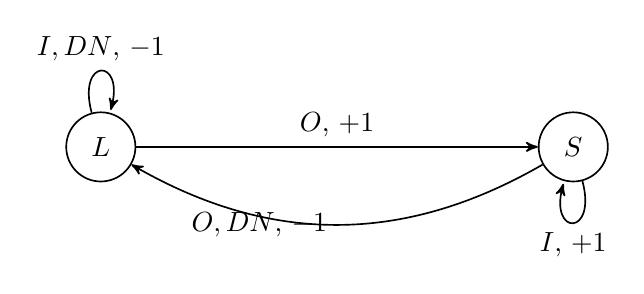
\begin{tikzpicture}[->,>=stealth',auto,node distance=6cm,semithick]
\tikzstyle{every state}=[text=black]
\node[state]         (L)			  {$L$};
\node[state]         (S) [right of=L] {$S$};


\path	(L) edge [loop above] node {$I, DN$, $-1$} (L)
		     edge node [bend right] {$O$, $+1$} (S) 
		 (S) edge [loop below] node {$I$, $+1$} (S)
		     edge [bend left] node [left] {$O, DN$, $-1$} (L);

\end{tikzpicture}		\\
\\


\subsection{Part (b)}

\subsubsection{Policy iteration}
\begin{itemize}
\item Let us assume an initial estimate of value function, $V_{0}=\{L:0,S:0\}.$

\item Initial Policy given as, $\pi_{0}=\{L:I,\,S:I\}$.
 
\item $p_{\pi_{0}}=\begin{array}{cc}
1 & 0\\
0 & 1
\end{array}$. $r_{\pi_{0}}=\begin{array}{c}
-1\\
+1
\end{array}$ $V_{\pi_{0}}=(I-\gamma p_{\pi_{0}})^{-1}r_{\pi_{0}}=\begin{array}{c}
-10\\
10
\end{array}$
\\The state value function in policy evaluation step forming a infinite gp ( sum of G.P with $a=1 ,r=0.9$ ).
\item Now, $\pi_{1}(L)=argmax_{a}\{O:\,1+0.9(10),I:-1+0.9(-10)\}=argmax_{a}\{O:10,I:-10\}=O$\\
$\pi_{1}(S)=argmax_{a}\{O:\,-1+0.9(-10),I:1+0.9(10)\}=argmax_{a}\{O:-10,I:10\}=I$\\
Therefore, $\pi_{1}=\{L:O,\,S:I\}$.
\item $p_{\pi_{1}}=\begin{array}{cc}
0 & 1\\
0 & 1
\end{array}$. $r_{\pi_{1}}=\begin{array}{c}
+1\\
+1
\end{array}$ $V_{\pi_{1}}=(I-\gamma p_{\pi_{1}})^{-1}r_{\pi_{1}}=\begin{array}{c}
10\\
10
\end{array}$
\item Now, $\pi_{2}(L)=argmax_{a}\{O:\,1+0.9(10),I:-1+0.9(10)\}=argmax_{a}\{O:10,I:8\}=O$\\
$\pi_{2}(S)=argmax_{a}\{O:\,-1+0.9(10),I:1+0.9(10)\}=argmax_{a}\{O:8,I:10\}=I$\\
Therefore, $\pi_{2}=\{L:O,\,S:I\}$.
\item $\pi_{1}=\pi_{2}.$ Thereforce, policy iteration converged to the
optimal policy $\pi^{*}=\{L:O,\,S:I\}.$
\item And optimal value function $V^{*}=V_{\pi_{1}}=\{L:10,S:10\}.$
\end{itemize}

\subsubsection{Value iteration}
\begin{itemize}
\item Let us assume an initial estimate of value function, $V_{0}=\{L:0,S:0\}.$
\item Now, $V_{1}(L)=max_{a}\{O:1+0.9(0),I:-1+0.9(0)\}=1$.\\
$V_{1}(S)=max_{a}\{O:-1+0.9(0),I:1+0.9(0)\}=1.$
\item $V_{2}(L)=max_{a}\{O:1+0.9(1),I:-1+0.9(1)\}=1.9$.\\
$V_{2}(S)=max_{a}\{O:-1+0.9(1),I:1+0.9(1)\}=1.9.$
\item $V_{3}(L)=max_{a}\{O:1+0.9(1.9),I:-1+0.9(1.9)\}=2.71$.\\
$V_{3}(S)=max_{a}\{O:-1+0.9(1.9),I:1+0.9(1.9)\}=2.71.$
\item $V_{4}(L)=max_{a}\{O:1+0.9(2.71),I:-1+0.9(2.71)\}=3.439$.\\
$V_{4}(S)=max_{a}\{O:-1+0.9(2.71),I:1+0.9(2.71)\}=3.439.$
\item Following the trend, we can observe that $V^{*}$converges to $\{L:10,S:10\}$
( sum of G.P with $a=1,r=0.9$ ).
\end{itemize}

\subsection{Part (c)}

Now we know that $V^{*}=\{L:10,S:10\}$. Knowing this, we can compute
$Q^{*}(s,a)$ with one-step look ahead at $V^{*}$.\\
\\
$Q^{*}(L,O)=1+0.9V^{*}(S)=10$\\
$Q^{*}(L,I)=-1+0.9V^{*}(S)=8$\\
$Q^{*}(S,O)=-1+0.9V^{*}(L)=8$\\
$Q^{*}(S,I)=1+0.9V^{*}(L)=10$

\subsection{Part (d)}
At present it is Laughing state, To come to silent state one should follow the optimal policy. Play the organ then house become silent then burn the incense and continue it burning the house will remain silent forever.

\section{Solution: 3} 
Monte-Carlo and Policy gradient will work on Non Markovian problem setup also, whereas TD learning better work on Markovian scenario.
\\MC must wait until end of episode before return is known. MC only works for episodic (terminating) environments.MC does not exploit Markov property. Usually more effective in non-Markov environments.
\\TD can learn online after every step.TD can learn from incomplete sequences.TD works in continuing (non-terminating) environments. TD exploits Markov property. Usually more efficient in Markov environments.
\section{Solution: 4}
For the given grid-world we have, State set $=\{S,P,Q,T1,T2\}$.\\
\\
\\
\begin{tabular}{|c|c|c|c|c|}
\hline 
~~~ & ~~~ & ~S~ & ~~~ & ~~~\tabularnewline
\hline 
\hline 
T2 & {*} & P & Q & T1\tabularnewline
\hline 
\end{tabular}\\
\\
It is mentioned in the question for terminating on state $T1$ will get reward $+10$ and on terminating in state $T2$ will get $+5$, For state $*$ is $a$ units reward.\\
Below transition diagram shows all possible actions that can be taken on any state. there are 2 actions left and right in all three states $P$,$Q$ and $*$ total possibility of policies are 8. Now we calculate value function on all 4 states on 8 policies. choose policy which is better than all.\\
\\
\begin{tabular}{|c|c|c|c|c|}
\hline 
~~~ & ~~~ & ~$\downarrow$~ & ~~~ & ~~~\tabularnewline
\hline 
\hline 
$T2$ & $\begin{array}{c}
\leftarrow\\
\rightarrow
\end{array}$ & $\begin{array}{c}
\leftarrow\\
\rightarrow
\end{array}$ & $\begin{array}{c}
\leftarrow\\
\rightarrow
\end{array}$ & $T1$\tabularnewline
\hline 
\end{tabular}\\
\\

\subsection{Possibility 1}

\begin{tabular}{|c|c|c|c|c|}
\hline 
~~~ & ~~~ & ~$\downarrow$~ & ~~~ & ~~~\tabularnewline
\hline 
\hline 
$T2$ & $\begin{array}{c}
\leftarrow\end{array}$ & $\leftarrow$ & $\leftarrow$ & $T1$\tabularnewline
\hline 
\end{tabular}\\
\\

$S$ = $a\gamma+5\gamma^{2}$
\space\space 
$Q$ = $a\gamma+5\gamma^{2}$ 
\space\space
$P$ = $a+5\gamma$
\space\space
$*$ = $5$

\subsection{Possibility 2}

\begin{tabular}{|c|c|c|c|c|}
\hline 
~~~ & ~~~ & ~$\downarrow$~ & ~~~ & ~~~\tabularnewline
\hline 
\hline 
$T2$ & $\begin{array}{c}
\leftarrow\end{array}$ & $\leftarrow$ & $\rightarrow$ & $T1$\tabularnewline
\hline 
\end{tabular}\\
\\\\
\space\space $S$ = $a\gamma+5\gamma^{2}$
\space\space 
$Q$ = $10$
\space\space 
$P$ = $a+5\gamma$
\space\space 
$*$ = $5$


\subsection{Possibility 3}

\begin{tabular}{|c|c|c|c|c|}
\hline 
~~~ & ~~~ & ~$\downarrow$~ & ~~~ & ~~~\tabularnewline
\hline 
\hline 
$T2$ & $\begin{array}{c}
\leftarrow\end{array}$ & $\rightarrow$ & $\leftarrow$ & $T1$\tabularnewline
\hline 
\end{tabular}\\
\\\\
\space\space
$S$ = $0$
\space\space
$Q$ = $0$
\space\space
$P$ = $0$
\space\space
$*$ = $5$


\subsection{Possibility 4}

\begin{tabular}{|c|c|c|c|c|}
\hline 
~~~ & ~~~ & ~$\downarrow$~ & ~~~ & ~~~\tabularnewline
\hline 
\hline 
$T2$ & $\begin{array}{c}
\leftarrow\end{array}$ & $\rightarrow$ & $\rightarrow$ & $T1$\tabularnewline
\hline 
\end{tabular}\\
\\
\space\space
$S$ = $10\gamma^{2}$
\space\space	
$Q$ = $10$ 
\space\space
$P$ = $10\gamma$
\space\space
$*$ = $5$

\subsection{Possibility 5}

\begin{tabular}{|c|c|c|c|c|}
\hline 
~~~ & ~~~ & ~$\downarrow$~ & ~~~ & ~~~\tabularnewline
\hline 
\hline 
$T2$ & $\begin{array}{c}
\rightarrow\end{array}$ & $\leftarrow$ & $\leftarrow$ & $T1$\tabularnewline
\hline 
\end{tabular}\\
\\
\space\space	

$S$ = $\frac{a\gamma^{3}}{1-\gamma^{2}}$
\space\space $Q$ = $\frac{a\gamma^{3}}{1-\gamma^{2}}$
\space\space$P$ = $\frac{a\gamma^{2}}{1-\gamma^{2}}$
\space\space$*$ = $\frac{a\gamma}{1-\gamma^{2}}$\space\space

\subsection{Possibility 6}

\begin{tabular}{|c|c|c|c|c|}
\hline 
~~~ & ~~~ & ~$\downarrow$~ & ~~~ & ~~~\tabularnewline
\hline 
\hline 
$T2$  $\begin{array}{c}
\rightarrow\end{array}$ & $\leftarrow$ & $\rightarrow$ & $T1$\tabularnewline
\hline 
\end{tabular}\\
\\
\space\space
$S$ = $\frac{a\gamma^{3}}{1-\gamma^{2}}$
\space\space$Q$ = $10$
\space\space$P$ = $\frac{a\gamma^{2}}{1-\gamma^{2}}$
\space\space$*$ = $\frac{a\gamma}{1-\gamma^{2}}$\space\space
 

\subsection{Possibility 7}

\begin{tabular}{|c|c|c|c|c|}
\hline 
~~~ & ~~~ & ~$\downarrow$~ & ~~~ & ~~~\tabularnewline
\hline 
\hline 
$T2$ & $\begin{array}{c}
\rightarrow\end{array}$ & $\rightarrow$ & $\leftarrow$ & $T1$\tabularnewline
\hline 
\end{tabular}\\
\\
\space\space
$S$ = $0$
\space\space 
$Q$ = $0$
\space\space
 $P$ = $0$
\space\space
 $*$ = $0$
\space\space
 
\subsection{Possibility 8}

\begin{tabular}{|c|c|c|c|c|}
\hline 
~~~ & ~~~ & ~$\downarrow$~ & ~~~ & ~~~\tabularnewline
\hline 
\hline 
$T2$ & $\begin{array}{c}
\rightarrow\end{array}$ & $\rightarrow$ & $\rightarrow$ & $T1$\tabularnewline
\hline 
\end{tabular}\\
\\
\space\space
$S$ = $10\gamma^{2}$
\space\space
 $Q$ = $10$
\space\space
 $P$ = $10\gamma$
\space\space
 $*$ = $10\gamma^{2}$

\subsection*{Conclusion}

For optimal policy $\pi_{i}$ , $V_{\pi_{i}}(s)\geq max\,V_{\pi_{j}}(s)$
for $i\neq j$ for all states $s$. Use optimal policy rule for each
policy, we get the following results.
\begin{itemize}
\item Possibility $1$ and $2$ can never be optimal for any $\lambda$.
\item Possibility 4 and 8 will be optimal for a$\leq 0$.
\item  Policy 5 and 6  will be optimal for $\lambda >  \frac{\sqrt{a^2 + 400}-a}{20}.$
\item Policy 3 and 7 can never be optimal for any $\lambda$.	
\end{itemize}

\section{Solution: 5} 
Egocentric: Self to neighbor, Represents the location of agent in state space relative to its neighbor only.

\begin{itemize}
\item Assume state configuration in some group repeated in the state space then in this scenario Egocentric RL agent take advantage to learn the problem faster,
\item In egocentric state representation memory space can also be saved as the state space will reduced.
\item Where as similar scenario may be confusing also to the agent. Because it only relate things to its neighbor it don't know what will happen after some steps.
\item In Egocentric representation, Generalization is more difficult as compare to normal RL state space scenario. 
\end{itemize}

\section{Solution: 6}
There are some drawbacks in DP algorithm as when number of states are increases its complexity increases too much. To overcome this problem we use RTDP Algorithm which give preference to frequently used states. If we take advantage of symmetries ,it will account into less computation for solving the problem.
\\In RTDP we need a technique for sampling strategy on the basis of symmetry which take less time and tends to better algorithm than exists.
\subsection*{Algorithm}
We make groups of similar states based on the symmetries.
\begin{itemize}
\item Initialize $Q(s_t,a_t)=0 $  $\forall$ s $\forall$ a, for time t.
\item Sample a trajectory following a policy $\pi$.
\item At each time step t $(s_t,a_t)$ in the trajectory:
\begin{itemize}
\item if $(s_t,a_t)$ seen earlier that is exist in any symmetric group. we leave it and start the computation from fresh $(s_{t+1},a_{t+1})$
\item else sample it till we get terminal state.
\end{itemize}
\item Update all the states that are in symmetric group with the same value. $Q(s_t,a_t)=Q(s'_t,a'_t)$ if s and s' are in same symmetric group.
\item Other states have already there unique values from sampling. $Q(s,a)=R(s,a)+\Sigma\gamma P'(s,a,s')max_a{'}(s',a')$

\end{itemize}
\subsection*{Advantages}
\begin{itemize}
\item If RTDP need MDP in memory it will take less memory as we group out all symmetric states.

\item It is faster also as the state space is reduced.
\item This algorithm converge faster also as the update step, updates similar state at same time step. 
\end{itemize}
\section{Solution: 7} 
We will treat it as separate M MDP problems with each of size K.
\subsection{Problem representation}
$S={s_1,s_2, . . . . . ., s_m}$
where $s_i$ represent  state space of $i^th$ MDP.
\\$A={a_1,a_2, . . . . . ., a_m}$
where $a_i$ represent  action set of $i^th$ MDP.
Similarly Rewards and probability also defined.
The set is defined {S,A,R} for all M problems.
\section{Solution: 8} 
\subsection{Part (a)}
For the calculation of state values in First visit Monte Carlo we take first time vist of state in any episode and calculate its return in that episode. 
 state values .\\
\\
\begin{alignat*}{1}
V(A) & =\frac{(3)+(1)+(0)+(1)+(1)}{5}=6/5
\end{alignat*}
\\
\begin{alignat*}{1}
V(B) & =\frac{(2)+(0)+(1)+(0)+(0)+(1)}{6}=4/6
\end{alignat*}
\\
\begin{alignat*}{1}
V(C) & =\frac{(1)+(0)+(0)+(0)+(1)+(1)}{6}=3/6
\end{alignat*}


\subsection{Part (b)}
The state-transition diagram is shown below.State include there reward and on arrows transition probability mentioned.\\
\\
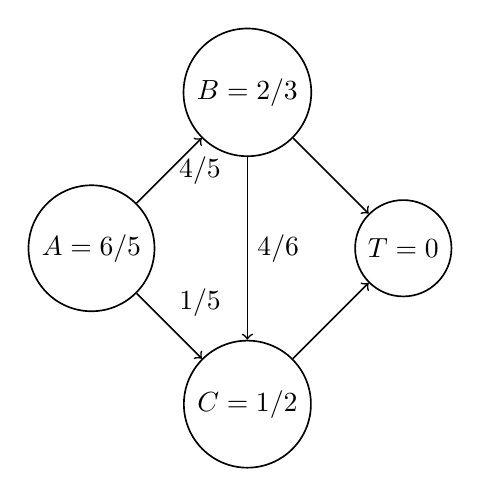
\begin{tikzpicture}[->,=> stealth',auto,node distance=2.8cm,semithick]
\tikzstyle{every state}=[text=black]
\node[state]         (A)					{$A=6/5$};
\node[state]         (B) [above right of=A] {$B=2/3$};
\node[state]         (C) [below right of=A] {$C=1/2$};
\node[state]         (T) [below right of=B] {$T=0$};


\path	(A) edge node		[right] {4/5} (B)
		     edge		node {1/5} (C)
		 (B) edge 	node {4/6} (C)
		     edge 	node {} (T)
		 (C) edge 	node {} (T);
\end{tikzpicture}	
\\
\\
\\
For calculating transition probabilities consider all episodes and average the no of transitions A->B , A->C, B->C, B->T, C->T. For reward calculation consider episode states reward and average them.   
\subsection{Part (c)}
Batch $TD(0)$ converged state values are calculated from MDP. BY solving simultaneous state value equations of each state.
\\
$V(T)=0.$ Based on transition probabilities,\\
\\
$V(A)=6/5 + 4/5V(B)+1/5V(C)$\\
\\
$V(B)=2/3+ 4/6V(C)$\\
\\
$V(C)=1/2$\\
\\
Solving the above system of equations, we get,\\
\\
\begin{tabular}{|c|c|}
\hline 
State $s$ & Value $V(s)$\tabularnewline
\hline 
\hline 
$A$ & $21/10$\tabularnewline
\hline 
$B$ & $1$\tabularnewline
\hline 
$C$ & $1/2$\tabularnewline
\hline 
$T$ & $0$\tabularnewline
\hline 
\end{tabular}


\section{Solution: 9}
Yes we can learn the value function of an arbitrary policy using the optimal policy.
We use SARSA or Monte Carlo as these are on-policy method and generate sample trajectory from them to calculate arbitrary policy.
\begin{itemize}
\item Be sure Q-values that are estimated must belong to arbitrary policy. For this we can use importance sampling to weigh the updates.
\item This method have high variance so we can use bias in important sampling to reduce it.
\item Optimal policy should cover the arbitrary police then only we can learn the value function.
\item Optimal policy must be stochastic wherever arbitrary policy is stochastic.
\end{itemize}

\section{Solution: 10} 
Reference: RL course Book\\\\

In question it is asked for a bandit problem in which the parameters on which the policy depends are the preference of the actions and the action selection probabilities which are determined by following softmax relationship-
\begin{alignat*}{1}
\pi_{t}(a_{j})= & \frac{e^{p_{t}(a_{j})}}{\sum_{i=1}^{n}e^{p_{t}(a_{i})}}
\end{alignat*}
\\
where n is the total number of actions and $p_{t}(a)$ is the preference value of action $a$ at time $t$.\\
The REINFORCE update equation is:\\
\\
\begin{alignat*}{1}
\theta_{t+1} & \leftarrow\theta_{t}+\alpha_{t}(r_{t}-b_{t})\nabla_{p_{t}}log(\pi_{t}(a_{t}))\frac{\partial p_{t}}{\partial\theta_{t}}
\end{alignat*}
$ $\\
where relation of $b_{t}$ and $b_{t+1}$ is given by $b_{t+1}=b_{t}+\beta(r_{t}-b_{t})$.\\
\\
solving both the equation we get,
\begin{alignat*}{1}
\theta_{t+1} & \leftarrow\theta_{t}+\alpha_{t}(r_{t}-b_{t})\{1-\pi_{t}(a_{t})\}\frac{\partial p_{t}}{\partial\theta_{t}}
\end{alignat*}


\section{Solution 11}
Reference: RL course book\\\\
Now for the same bandit problem we have parameters as the mean $\mu$ and variance $\sigma^{2}$ of the normal distribution. Action are chosen according these parameters and the baseline is considered here $b_{t}=0$..
\\
\begin{alignat*}{1}
\pi_{t}(a;\mu_{t},\sigma_{t})= & \frac{1}{\sqrt{2\pi\sigma}}e^{-\frac{(a-\mu_{t})^{2}}{\sigma_{t}^{2}}}
\end{alignat*}
\\
The REINFORCE update equation is:\\
\\
\begin{alignat*}{1}
\theta_{t+1} & \leftarrow\theta_{t}+\alpha_{t}(r_{t}-b_{t})\nabla_{\theta_{t}}log(\pi_{t}(a_{t}))
\end{alignat*}
\\
After considering $\theta_{t}$ as $ \begin{array}{c}
\mu_{t}\\
\sigma_{t}
\end{array}$ . \\We get separate equation for mean $\mu_t{t+1}$
and for $\sigma_{t+1}$

\begin{alignat*}{1}
\mu_{t+1} & \leftarrow\mu_{t}+\alpha_{t}r_{t}(a_{t}-\mu_{t})
\end{alignat*}

\begin{alignat*}{1}
\sigma_{t+1} & \leftarrow\sigma_{t}+\frac{\alpha_{t}r_{t}\{(a_{t}-\mu_{t})^{2}-\sigma_{t}^{2}\}}{\sigma_{t}}
\end{alignat*}

%\begin{figure}[htb!]\includegraphics[width=\textwidth]{cnn.jpg}
%\caption{CNN architecture}
%\end{figure}

\begin{comment}
\newpage
\section{Question Answer}
\begin{figure}[htb!]
%\includegraphics[width=\textwidth]{answer2.jpeg}
\end{figure}
\newpage
\section{Question Answer}
Plots of Histogram
\subsection{Answer }
\end{comment}
\end{document}
